%%%%%%%%%%%%%%%%%%%%%%%%%%%%%
% En-tête classique
%%%%%%%%%%%%%%%%%%%%%%%%%%%%%

%\documentclass[10pt,a4paper]{article}%           autres choix : report, book
\documentclass[11pt,a4paper]{scrartcl}%           autres choix : report, book

\usepackage[utf8]{inputenc}%       encodage du fichier source
\usepackage[T1]{fontenc}%          gestion des accents (pour les pdf)
\usepackage[frenchb]{babel}%        rajouter éventuellement english, greek, etc.
%\usepackage[english]{babel}%        rajouter éventuellement english, greek, etc.
\usepackage{textcomp}%             caractères additionnels
%\usepackage{mathtools,mathtext}
\usepackage{amsmath,amssymb,amsopn,amsthm}%      pour les maths
\usepackage{lmodern}%              remplacer éventuellement par txfonts, fourier, etc.
\usepackage[a4paper]{geometry}%    taille correcte du papier
\usepackage{graphicx}%             pour inclure des images
\usepackage{xcolor}%               pour gérer les couleurs
\usepackage{microtype}%            améliorations typographiques
\usepackage{tikz}
\usepackage{graphicx}
%\includegraphics
\usepackage{hyperref}%             gestion des hyperliens
\hypersetup{pdfstartview=XYZ}%     zoom par défaut


\theoremstyle{plain}
\newtheorem{theoreme}{Thèoréme}[section]
\newtheorem{corollaire}[theoreme]{corollaire}
\newtheorem{proposition}[theoreme]{proposition}
\newtheorem{lemme}[theoreme]{lemme}
\newtheorem{exple}{Exemple}
\newtheorem{exo}{Exercice}
\theoremstyle{definition}
\newtheorem{definition}[theoreme]{Definition}
\theoremstyle{remark}
\newtheorem*{remarque}{Remarque}
\newcommand{\N}{\mathbb{N}}
\newcommand{\Z}{\mathbb{Z}}
\newcommand{\R}{\mathbb{R}}
\newcommand{\C}{\mathbb{C}}
\newcommand{\K}{\mathcal{C}}
\newcommand{\norme}[1]{\left\lVert#1\right\rVert}% Pour la norme
\newcommand{\va}[1]{\left\lvert#1\right\rvert}%pour la valeur absolue
\newcommand{\mtext}[1]{\quad\text{#1}\quad}% pour écrire du texte séparé par deux grands espaces en mode mathématique.
\newcommand{\abs}[1]{\lvert#1\rvert_{\mathcal{A}}}% pour les v.a


%\title{}
% \author{DHIYAOU-DINE Ahmed Kassim}
% \date{}
%%%%%%%%%%%%%%%%%%%%%%%%%%%%%%%%%%%%%%%%%%%%%%%
%recup inserer code
%%%%%%%%%%%%%%%%%%%%%%%%%%%%%%%%%%%%%%%%%%%%%%%
%% http://www.cnam.fr/maths/Membres/ghorbanzadeh/
 
\usepackage[francais]{babel} 
\usepackage{fancyvrb}
\usepackage{xcolor}

\definecolor{Zgris}{rgb}{0.87,0.85,0.85}

\newsavebox{\BBbox}
\newenvironment{DDbox}[1]{
\begin{lrbox}{\BBbox}\begin{minipage}{\linewidth}}
{\end{minipage}\end{lrbox}\noindent\colorbox{Zgris}{\usebox{\BBbox}} \\
    [.5cm]}
\begin{document}
	
 \begin{titlepage}
	\hspace*{-10mm}
	
	%\vspace*{-20mm}		\includegraphics[width=30mm]{logo-utlnn}
	%\hspace*{+90mm}		\includegraphics[width=30mm]{logo-lsis}
	
	
	\vspace*{20mm}
	\begin{center}
		
		\textbf{\LARGE Projet de Modélisation pour les énergie\\ Promotion M2 MACS 2019-2020}\\ [2cm]
		%titre
		%\HRule \\ [0.5cm]
		{\huge \bfseries  Schéma VF4 pour un problème de diffusion \\ [0.4cm] }
		%	\HRule \\ [2cm]
		\vspace*{+40mm}
		\begin{minipage}{0.4\textwidth}
			\begin{flushleft} \large
				\emph{Nom étudiant:}\\ \textsc{Dhiyaou-dine AHMED KASSIM} 
			\end{flushleft}
		\end{minipage}
		\hspace*{+26mm} \vspace*{+40mm}
		\begin{minipage}{0.4\textwidth}
			\begin{flushleft} \large
				\emph{Enseignant:}\\ \textsc{MAZEN Saad}
			\end{flushleft}
		\end{minipage}
		\vfill
		{\large   Mars 2020}
	\end{center}
\end{titlepage}
	

\textbf{Schéma VF4-Problème de diffusion}\\
Le but de ce $TP$ est de programmer la méthode de 		volumes finis $VF4$ sur un maillage triangulaire orthogonale. On considère l'équation elliptique suivante :
\begin{equation}
-\Delta u(x) +\theta u(x) = f(x), x \in \Omega
\end{equation}
avec la condition aux limites suivantes : 
\begin{equation}
u(x) = g, x \in \partial_{\Omega}
\end{equation}
\begin{itemize}
\item[$1)$] Gestion du maillage
Le maillage de type \textbf{MAILLAGEGEO} (dans le fichier Lestests.f90) contient les informations nécessaires pour construire un maillage :
	\begin{itemize}
	\item nombre des sommets \textbf{Nbs}
	\item nombre des triangles \textbf{Nbt}
	\item nombre de segments \textbf{Nseg}
	\item nombre des sommets intérieurs \textbf{Nbord}
	\item Les coordonnées de tous les sommets CoordS(1 :2,1 :Nbs) et le type des sommets $0$ pour un sommet à l’intérieur du domaine et 1 s’il est sur le bord.
	\item Pour chaque triangle, les numéros des trois sommets NuSo(1 :3,1 :Nbt), les coordonnées
du centre CoordK, aire AireK
	\item Pour chaque segment, les numéros des deux sommets NuSeg(1 :2, . ), le nombre des voisins $NombVoisSeg =2$ si le segment à l’intérieur et 1 s’il est sur le bord, les numéros des deux triangles de part et d’autre du segment, NumTVoisSeg(1 :2) avec NumTVoisSeg(2) négatif si le segment est sur le bord, le type du segment $NTypSeg( :) =0$ si le segment est à l’intérieur et 1 s’il est sur le bord, TauKL et enfin $dKL$
	\item Le programme principal est flaplacienvfmacs.f90. Avant de commencer à programmer, ouvrir chaque module longr, parmmage, imprime, intmatvec, algebrelineaire, plotvtkmod et comprendre sans les modifier. Le module fsourcemod peut être modifier.
Le programme principal contient toutes les étapes commentées.
	\item La subroutine init contient les données et donc modifiable.
	\item Comprendre la subroutine readmesh(nonmodifiable)
	\item La structure de la matrice A est celle du stockage creux classique : les coefficients non
nuls de $A$, indice premier dans la ligne, indice de colonne. La subroutine matrixinitVF4 (non
modifiable) alloue la structure de la matrice à comprendre absolument pour comprendre le
reste !
	\item Le second membre est : $|K|f (x_K )$, compléter l’instruction $A\%F$. 
   	\item $A\%Bg$ contient le second membre et la contribution sur le bord.
	\item Expliquer la subroutine $assembleVF4$ et la compléter.
	\item Expliquer la subroutine assembletheta
	\item compléter le fichier fsoucemod pour tester le code avec les solutions exactes solutions :
		\begin{itemize}
			\item[$(a)$] $ChoixPb = 1$, $Uexacte = 1$
			\item[$(b)$] $ChoixPb = 2$, $Uexacte = x + y$
			\item[$(c)$] $ChoixPb = 3$, $Uexacte = x^2 - y^2$
			\item[$(d)$] $ChoixPb = 4$, $Uexacte = \cos(5\pi(x + y))$
			\item[$(e)$] $ChoixPb = 5$, $Uexacte = x(1 - x)y(1 - y)$
			\item[$(f)$] $Choixpb = 6$, $Uexacte = \sin(\pi x)\sin(\pi y)$
		\end{itemize}
	\item \textbf{Réponse aux questions}
		\begin{itemize}
			\item On complète l'instruction $A\%F$ :\\
			
		\begin{DDbox}{\linewidth}
		\begin{Verbatim}
    A%F = 0.D0 
    DO i = 1, Nbt	
      A%F (i) = fsource(CoordK(1,i),CoordK(2,i),choixpb )  
    END DO
		\end{Verbatim}
		\end{DDbox}
		\item Explication du subroutine $assembleVF4.f90$\\
		Dans cette subroutine nous assemblons la contribution de diffusion et de l'opérateur $-\Delta u(x)$ en dimension $2$. C'est à dire $-d(\frac{d^2u}{dx^2} + \frac{d^2u}{dy^2}$  par la méthode volumes finis VF4. On a besoin de la subroutine $imprime.f90$ qui sert à écrire les résultats dans un fichier, à fin de pouvoir les utiliser pour résoudre le problème. Le fichier en question affiche les résultats relatifs à chaque élément du maillage. Elle utilise aussi la subroutine$longr.f90$ et $parmmage.f90$ qui contiennent les déclaration de nos variables et en fin $fsource.f90$ contient les solutions exactes en fonction du problème choisi.\\
		La subroutine $assembleVF4.f90$, dans le cas de \textbf{Dirichlet} parcours, les deux sommets de chaque segment, en fonction de l'élément sur lequel on se trouve, le triangle voisin et avec ses deux éléments, elle fait appel à la fonction $Ajout$ pour ajouter les contributions de chaque élément.  qui seront ensuite écrit sur  $imprime.f90$. Après il rajoute les conditions aux bords. Dans le cas de \textbf{Neumann} homogène, le flux est nul aux bords. Sinon il faut modifier $A\%Bg$, qui sert à rajouter les conditions aux bords. EN fin il va placer tous ces contributions dans la matrice globale.\\
Après compréhension des subroutines nécessaires on a :\\
			\begin{DDbox}{\linewidth}
			\begin{Verbatim}
 			!! contribution dans la ligne ik
        CALL Ajout (ik, ik, Coef_diffusion*TauKL(iseg),  A )

        CALL Ajout (ik, jL, -Coef_diffusion*TauKL(iseg), A  ) 

        !! contribution dans la ligne jL

        CALL Ajout ( jL, jL, Coef_diffusion*TauKL(iseg), A ) 
        CALL Ajout (jL, ik, -Coef_diffusion*TauKL(iseg), A )
		\end{Verbatim}
		\end{DDbox}
		\item La subroutine $assembletheta$, utilise les subroutines $longr.f90$, $imprime.f90$ et $parmmage.f90$ dont l'utilité est expliqué précédemment.
		\item Calcul de l'erreur $L^2$ entre la solution exacte et la solution calculée. Pour tracer les solution on travaille avec le maillage $MAILLAGEGEO3$\\
		\begin{DDbox}{\linewidth}
		\begin{Verbatim}
        ErreurL_2 = 0.
        DO i = 1, Nbt
          ErreurL_2 = ErreurL_2 + AireK(i)*(U(i)-Uexacte(i))**2
        END DO
		\end{Verbatim}
		\end{DDbox}
		\item Erreur pour un $Uexacte = x*x - y*y $ :\\
		
		$Erreur infiny  :    2.0531479375457407E-004$\\
		$Erreur infiny relative :    2.0977245849764911E-004$\\
		$Erreur L^2 :    1.0000000000035121     $\\
		$Max solution exacte :   0.97875000000000001     $\\
		$Max solution calculee :   0.97869941335201893   $ \\ 
		$Min solution exacte :  -0.97875000000000001    $ \\
		$Min solution calculee :  -0.97869941335201882 $
		
		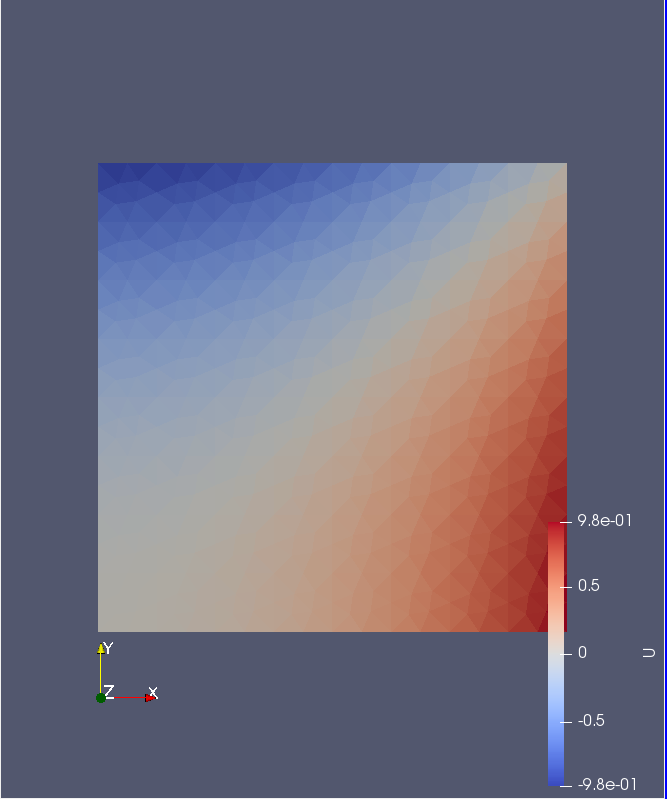
\includegraphics[width=7cm]{Ucalcule3}
		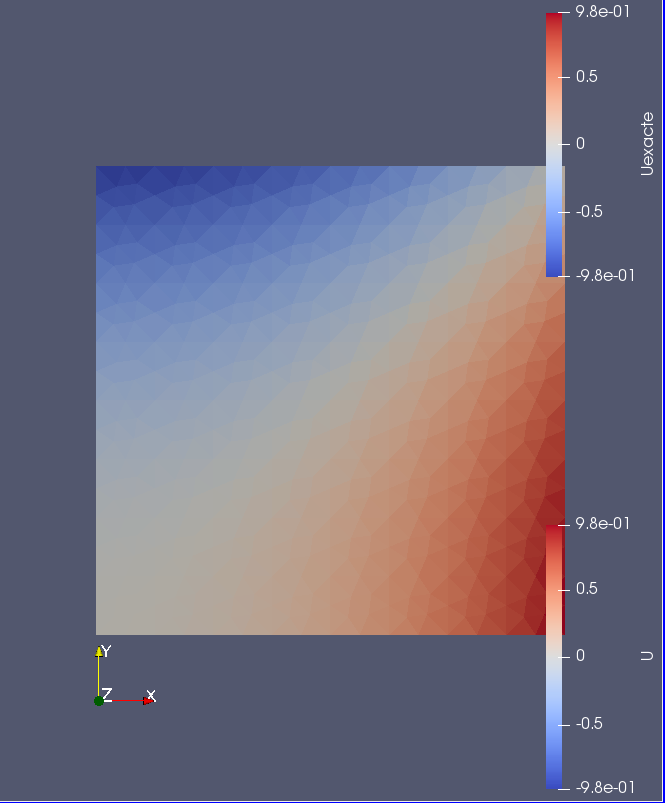
\includegraphics[width=7cm]{Uexacte3}\\
		

		\item Erreur pour un $ Uexacte = \cos(5.*\pi*(x+y)) $ :
			
		$Erreur infiny  :    1.1812723147457049$ \\    
		$Erreur infiny relative :    1.1869879863367347$\\     
		$Erreur L^2 :    1.0006824820349205     $\\
		$Max solution exacte :   0.99518472667219704$\\     
		$Max solution calculee :   0.89882812857500372$\\     
		$Min solution exacte :  -0.99518472667219693   $ \\ 
		$Min solution calculee :  -0.80860945075824686$ 
	 
		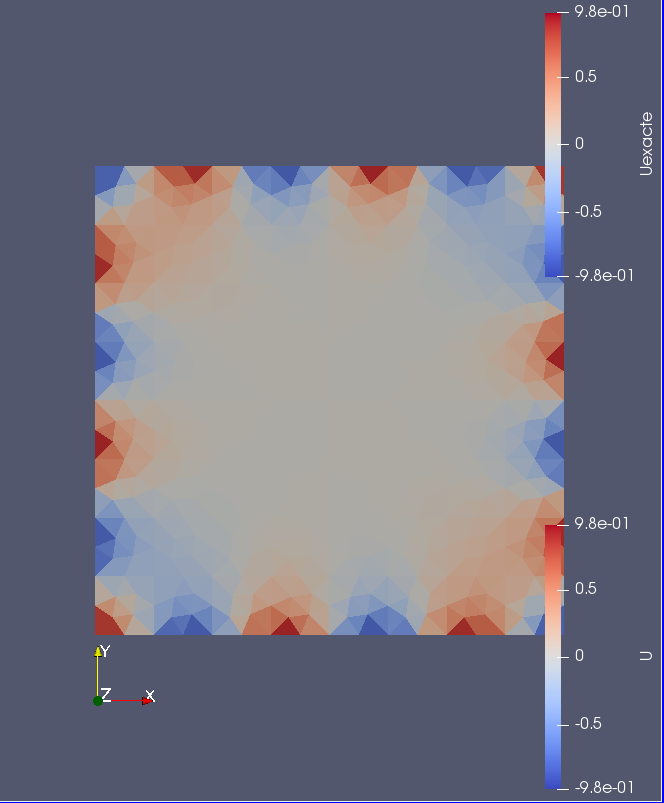
\includegraphics[width=7cm]{Ucalcule4}
		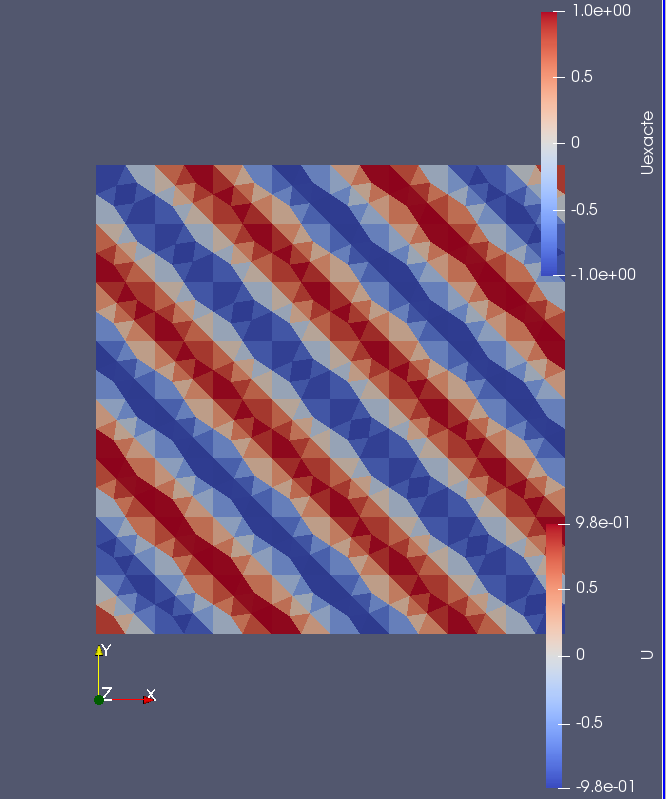
\includegraphics[width=7cm]{Uexacte4}\\
		\end{itemize}

	\end{itemize}
\end{itemize} 
\end{document}
